%This is an example for a chapter, additional chapter can be added in the skeleton-thesis
%To generate the final document run latex, build and quick build commands on the skeleton-thesis file not this one.
%This is chapter 2, the default skeleton thesis expects 2 chapters
\chapter{Design and Implementation}
\label{sec:method}
\toolname, a system for evaluating how removing permissions impacts the behavior of Android applications, was designed for the purpose of this study.  To evaluate each application, \toolname\ automatically runs the application, supplies it with various UI events, detects when the application crashes, and logs the cause of the crash.  
\toolname\ consists of the following components (see Figure \ref{fig:diagram}):

\begin{figure*}[t]
\centerline{\resizebox{0.8\linewidth}{!}{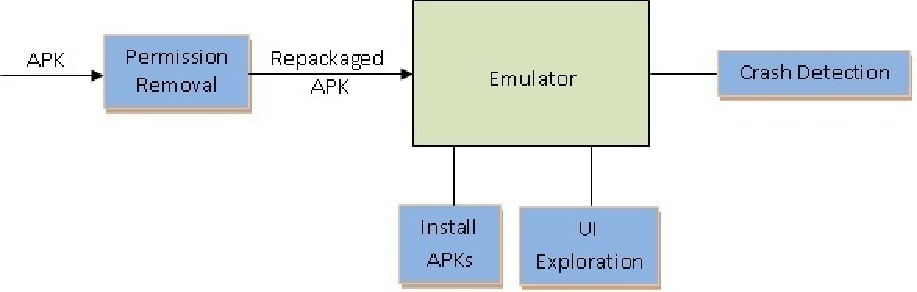
\includegraphics{flowchart}}}
\caption{PyAndrazzi Component Diagram}
\label{fig:diagram}
\end{figure*}

\paragraph{\bfseries Permission Removal}
\toolname\ decodes the application's APK file using APKTool.  Then, it removes the permission being evaluated.  Finally, it rebuilds the APK and signs it using Android's built-in debug key.

\paragraph{\bfseries Installation and Execution}
\toolname\ installs and runs applications in emulators.  It utilizes the MonkeyRunner framework to install and uninstall applications, provide UI inputs, and take screen shots of applications.

\paragraph{\bfseries Automatic UI Exploration}
\toolname\ needs to execute as much code as possible to maximize the number of adverse effects resulting from permission removal.  For each application, \toolname\ determines the list of activities and executes each one starting with the \texttt{Main} activity. During each activity, \toolname\ takes a screenshot and performs a series of screen touches.  This functionality is implemented using a UI introspection approach based on the AndroidViewClient library~\cite{Milano}.  Using this method, \toolname\ is able to query the screen for click-able elements and performs "random" touches with a high probability of changing the application state.

\paragraph{\bfseries Crash Detection}
\toolname\ needs to detect application crashes and their causes.  It uses ADB to access logcat, which provides us with the logs from the emulator, including system status and application crashes.  When an application crashes due to a fatal error, such as a \texttt{SecurityException}, a separate thread monitoring the logs will notify the testing thread, which will record the cause of the crash and launch the next Activity.



